% Technical companion to the fresnel-reduction-validation repository.
% Build: latexmk -pdf main.tex   (or upload this folder to Overleaf as-is)
\documentclass[11pt,a4paper]{article}

\usepackage[T1]{fontenc}
\usepackage[utf8]{inputenc}
\usepackage{lmodern}
\usepackage{microtype}
\usepackage[margin=2.4cm]{geometry}
\usepackage{amsmath,amssymb,bm}
\usepackage{graphicx}
\usepackage{booktabs}
\usepackage{array}
\usepackage{xcolor}
\usepackage{enumitem}
\usepackage[font=small,labelfont=bf]{caption}
\usepackage[colorlinks=true,linkcolor=blue!50!black,citecolor=blue!50!black,urlcolor=blue!50!black]{hyperref}

\graphicspath{{figures/}}
\setlength{\parskip}{0.35em}

% ---------------------------------------------------------------- macros
\newcommand{\mS}{\mathbf{S}}
\newcommand{\mSd}{\tilde{\mathbf{S}}}
\newcommand{\mR}{\mathbf{R}}
\newcommand{\mPhi}{\boldsymbol{\Phi}}
\newcommand{\mPsi}{\boldsymbol{\Psi}}
\newcommand{\mM}{\mathbf{M}}
\newcommand{\mI}{\mathbf{I}}
\newcommand{\mB}{\mathbf{B}}
\newcommand{\vc}{\mathbf{c}}
\newcommand{\vE}{\mathbf{E}}
\newcommand{\vF}{\mathbf{F}}
\newcommand{\vb}{\mathbf{b}}
\newcommand{\vh}{\mathbf{h}}
\newcommand{\vn}{\mathbf{n}}
\newcommand{\wi}{\boldsymbol{\omega}_i}
\newcommand{\wo}{\boldsymbol{\omega}_o}
\newcommand{\lam}{\lambda}
\newcommand{\diag}{\operatorname{diag}}
\newcommand{\dE}{\Delta E_{2000}}
\newcommand{\transp}{^{\mathsf{T}}}
\newcommand{\file}[1]{\texttt{#1}}
\newcommand{\code}[1]{\texttt{#1}}

\title{Reduced Conductor Fresnel for Real-Time Rendering\\
       \large Technical companion to the \file{fresnel-reduction-validation} repository}
\author{Mohammed Douidy\\ \small Master's internship, supervised by Pascal Barla \& Morgane Gerardin}
\date{September 2026}

\begin{document}
\maketitle

\begin{abstract}
\noindent
This document describes what the repository computes and how each quantity is
validated against a full spectral render.  The subject is an extension of the
non-orthogonal spectral reduction of Fichet, Belcour \& Barla (2024), which
covers angle-independent operators, to the angle-dependent specular Fresnel of
a conductor.  The Fresnel operator is factored on the four universal angular
basis functions of Belcour, Bati \& Barla (2020), giving a $3\times3$ matrix
$\mM_F(\theta)=\sum_i b_i(\theta)\mPhi_i$ applied to transported radiance.
The theory as implemented is in Sections~\ref{sec:reduction}
to~\ref{sec:synthesis}, the validation in Sections~\ref{sec:renderers}
and~\ref{sec:results}, the analysis of the residual error in
Section~\ref{sec:tint}, and the limitations in Section~\ref{sec:limits}.
\end{abstract}

\tableofcontents

% ======================================================================
\section{Scope and reading guide}
\label{sec:scope}

The reduction of Fichet et al.\ collapses an $N$-wavelength linear operator
into a $K\times K$ matrix ($K=3$ for XYZ) so that colour transport can run in a
tristimulus renderer.  Its published form applies to operators that are
diagonal in wavelength and independent of direction: albedo, transmittance,
fluorescent reradiation.  The specular reflectance of a metal is neither
separable that way nor negligible: the Fresnel term $F(\theta,\lam)$ depends
jointly on angle and wavelength, and it is the only wavelength-dependent factor
of a microfacet BRDF.

The idea validated here is to make it separable.  Belcour et al.\ (2020) showed
that for any physical conductor the angular curve $\cos\theta\mapsto
F(\cos\theta)$ lies in a four-dimensional subspace with universal basis
functions $b_0..b_3$.  Applying that per wavelength writes
$F(\theta,\lam)=\sum_i c_i(\lam)\,b_i(\theta)$, and each $c_i(\lam)$ is exactly
the kind of operator Fichet's reduction handles.  Four fixed $3\times3$
matrices per material, four scalar weights per pixel.

The repository answers three questions with numbers:
\begin{enumerate}[nosep]
  \item Is the \emph{angular} decomposition accurate for gold, inside a
        renderer?  (Yes: $\dE\approx0.02$--$0.04$ against a spectral
        reference.)
  \item Is the \emph{reduced matrix} accurate?  (Not to target: a systematic
        tint of $\dE\approx2$--$2.7$ under smooth illuminants, $0.8$ under a
        fluorescent lamp.)
  \item Where does that tint come from, and what would remove it?  (It is the
        metameric black of the illuminant folded into the visible by the
        material; anchoring the reconstruction operator on smooth spectra
        removes it at no runtime cost, and the matrix form is what keeps that
        stable over bounces.)
\end{enumerate}
Throughout, spectra are column vectors on a 1\,nm grid from 380 to 780\,nm
($N=401$), matrices act on the left, and $\theta$ is the angle between the
incident direction and the microfacet normal (half vector).

% ======================================================================
\section{Spectral reduction of a wavelength-only operator}
\label{sec:reduction}

\subsection{Basis, dual basis, reduced operator}

Let $\mS\in\mathbb{R}^{N\times3}$ hold the CIE~1931 colour-matching functions
as columns.  A spectrum $\vE$ has coordinates $\vc=\mS\transp\vE$; the dual
basis
\begin{equation}
  \mSd=\mS\,(\mS\transp\mS)^{-1},\qquad \mS\transp\mSd=\mI_3,
  \label{eq:dual}
\end{equation}
reconstructs from coordinates the unique spectrum in $\operatorname{span}\mSd$
with those coordinates.  For a wavelength-diagonal operator $\diag(f)$ the
reduced operator is
\begin{equation}
  \mPhi=\mS\transp\diag(f)\,\mSd\in\mathbb{R}^{3\times3},
  \qquad \vc_{\text{out}}=\mPhi\,\vc_{\text{in}},
  \label{eq:reduce}
\end{equation}
exact whenever $\vE\in\operatorname{span}\mSd$ and otherwise in error by the
part of $\vE$ the basis cannot see.  Section~\ref{sec:tint} makes that part
precise; it accounts for the entire residual.

\subsection{Normalisation, and why it differs from the fluorescence work}
\label{sec:norm}

\file{compute\_cmf.py} samples $\mS$ from Mitsuba's own internal CMF table
(\code{mi.cie1931\_xyz}) and divides all three columns by the \emph{single}
sum of the $\bar y$ column.  This differs from the per-column normalisation used in the sibling reflectance/fluorescence
repository.  Per-column normalisation applies three different gains and would
introduce a fixed per-channel tint relative to the spectral film's own
XYZ conversion, which uses one common factor.  \file{check\_conventions.py}
proves the stored $\mS$ equals Mitsuba's table exactly and that the hardcoded
IEC~61966-2-1 XYZ$\to$sRGB matrix equals \code{mi.xyz\_to\_srgb} to
$8.6\times10^{-5}$.  Both checks exit non-zero on failure.  The two
repositories' $\mS$ matrices are therefore not interchangeable, and $\mPhi$ is
invariant to a common rescaling of $\mS$ but not to a per-column one.

% ======================================================================
\section{Conductor Fresnel and its angular decomposition}
\label{sec:fresnel}

\subsection{Exact Fresnel}

A conductor is described by a complex index $\hat n(\lam)=\eta(\lam)+i\kappa(\lam)$.
For unpolarised light at incidence $\theta$,
\begin{align}
  a^2+b^2 &= \sqrt{(\eta^2-\kappa^2-\sin^2\theta)^2+4\eta^2\kappa^2},\\
  R_s &= \frac{a^2+b^2-2a\cos\theta+\cos^2\theta}{a^2+b^2+2a\cos\theta+\cos^2\theta},\qquad
  R_p = R_s\,\frac{a^2+b^2-2a\sin\theta\tan\theta+\sin^2\theta\tan^2\theta}
                 {a^2+b^2+2a\sin\theta\tan\theta+\sin^2\theta\tan^2\theta},\\
  F(\theta,\lam) &= \tfrac12\,(R_s+R_p).
\end{align}
\file{fresnel\_tools.py} implements exactly this (it is the evaluation routine
from the authors' helper module, reduced to the functions used).
\file{load\_ior.py} resamples gold's $\eta,\kappa$ from a two-block CSV in
micrometres onto the 1\,nm grid and asserts plausible values at 550\,nm.

\subsection{The four universal basis functions}
\label{sec:basis}

Belcour et al.\ (2020) build a corpus of normalised Fresnel curves
$\tilde F(\cos\theta)=\big(F(\cos\theta)-F(1)\big)/\big(1-F(1)\big)$ over a
large set of dielectric and conductor IORs, and extract by a two-pass SVD a
basis $\{b_0\equiv1,\;b_1,\;b_2,\;b_3\}$ on a 1000-point $\cos\theta$ grid such
that every physical curve is well approximated by four coefficients
(Figure~\ref{fig:basis}).  \textbf{This repository does not re-derive the
basis}: \file{extract\_basis.py} parses the table
\code{fresnel\_curves[1000][4]} from the authors' published Mitsuba plugin
source (\file{data/belcour2020/fresnel\_curves.hpp}) together with the two
probe indices their coefficient solve uses.  $b_1$ is the SVD-extracted first
mode, not the Schlick $(1-\cos\theta)^5$ it resembles; the two differ by up to
$0.12$ at grazing, and using Schlick in one place and the extracted $b_1$ in
another was a bug found and fixed during the work.

\subsection{Per-wavelength coefficients}
\label{sec:coeffs}

At a fixed $\lam$ the decomposition is
\begin{equation}
  F(\cos\theta,\lam)\;\approx\;\sum_{i=0}^{3}c_i(\lam)\,b_i(\cos\theta),
  \qquad
  c_0=F(1),\quad c_1=\max(1-c_0,\,0),
\end{equation}
and $c_2,c_3$ are the solution of the $2\times2$ system obtained by matching
the residual $F-c_0-c_1b_1$ at two probe angles ($\cos\theta_1=0.1201$,
$\cos\theta_2=0.4344$, the arg-max positions of $b_2$ and $b_3$), solved by
Cramer's rule exactly as in the authors' \code{fresnelToCoeffs()}.
\file{compute\_coeffs.py} does this for each of the 401 wavelengths and checks
the reconstruction at 550\,nm against the exact curve over all 1000 angles:
\textbf{maximum absolute error $0.0036$} (Figure~\ref{fig:coeffs}), guarded by
an assertion at $0.01$.

\begin{figure}[t]\centering
\begin{minipage}[t]{0.49\linewidth}\centering
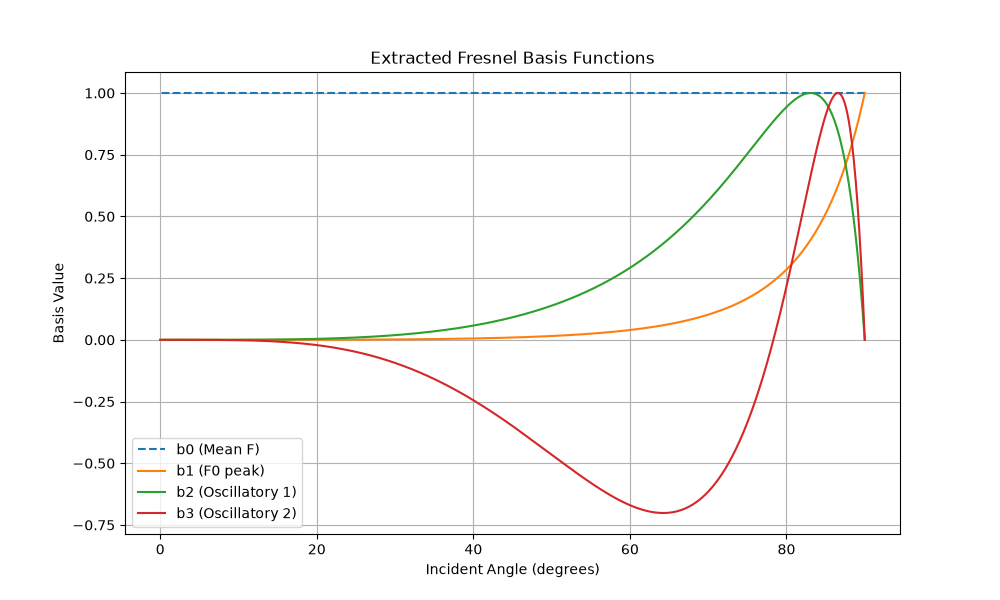
\includegraphics[width=\linewidth]{basis.png}
\caption{The four universal angular bases read from the authors' table.
$b_0\equiv1$; $b_3$ is negative over most of its range, which matters for how
it is stored on the GPU (Section~\ref{sec:godot}).}
\label{fig:basis}
\end{minipage}\hfill
\begin{minipage}[t]{0.49\linewidth}\centering
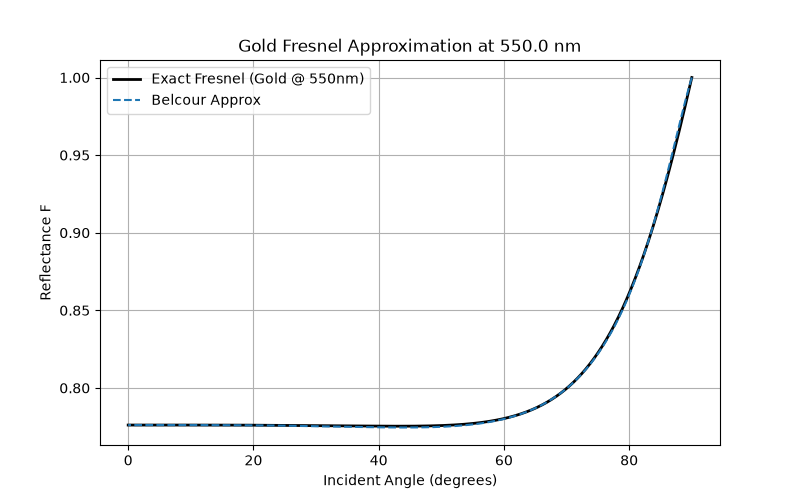
\includegraphics[width=\linewidth]{coeffs.png}
\caption{Exact conductor Fresnel of gold at 550\,nm and its four-coefficient
reconstruction.}
\label{fig:coeffs}
\end{minipage}
\end{figure}

% ======================================================================
\section{The synthesis: reduced Fresnel matrices}
\label{sec:synthesis}

\subsection{Separating angle from wavelength}

Each coefficient function $c_i(\lam)$ is a wavelength-only operator, so
Eq.~\eqref{eq:reduce} applies to it:
\begin{equation}
  \mPhi_i=\mS\transp\diag\!\big(c_i(\lam)\big)\,\mSd\in\mathbb{R}^{3\times3},
  \qquad i=0..3,
  \label{eq:phi}
\end{equation}
computed in \file{compute\_phi.py} as \code{(S.T * c[i]) @ Sb} without
materialising the diagonal.  The reduced Fresnel operator at any angle is then
\begin{equation}
  \boxed{\;\mM_F(\theta)=\sum_{i=0}^{3}b_i(\theta)\,\mPhi_i\;}
  \qquad \vc_{\text{out}}=\mM_F(\theta)\,\vc_{\text{in}} .
  \label{eq:MF}
\end{equation}
Angle enters only through four scalars and wavelength only through four
constant matrices.  The operator is therefore cheap (one basis fetch, four
$3\times3$ multiply-adds, one matrix-vector product) and can be
preintegrated.  The $b_i$ are universal; only the $\mPhi_i$ change with the
material.  \file{compute\_phi.py} checks that under a flat white illuminant at
$\cos\theta=0.5$ the reflected luminance is positive, below the incident
luminance, and larger than the reflected $Z$ (gold is yellow-orange).

\subsection{Split-sum preintegration for image-based lighting}
\label{sec:splitsum}

For a rough surface under distant lighting the specular integral factors, in
the split-sum approximation of Karis (2013), into a prefiltered environment
term and a preintegrated BRDF term.  Because the $b_i$ are scalar and
universal, the BRDF term is preintegrated once per basis:
\begin{equation}
  \bar b_i(\cos\theta_o,\alpha)=\int_\Omega b_i(\wi\!\cdot\!\vh)\,
  \frac{D(\vh;\alpha)\,G_2(\wi,\wo;\alpha)}{4\,(\wo\!\cdot\!\vn)}\,d\wi ,
  \qquad
  \bar{\mM}_F(\cos\theta_o,\alpha)=\sum_i\bar b_i\,\mPhi_i .
  \label{eq:bbar}
\end{equation}
\file{compute\_split\_sum.py} estimates each $\bar b_i$ on a $256\times256$
grid in $(\cos\theta_o,\alpha)$ with 4096 Halton samples per cell,
importance-sampling the GGX visible normal distribution (Heitz 2018).  The
per-sample weight reduces to $G_1(\wi)\,(\wi\!\cdot\!\vh)/(\wo\!\cdot\!\vh)$
because the VNDF density cancels $D$ and $G_1(\wo)$ algebraically.  The
$b_0$ channel is the ordinary $F{=}1$ GGX directional albedo and serves as a
sanity check (asserted near~1 at normal incidence and low roughness, and below
1 elsewhere).  Figure~\ref{fig:splitsum} shows the four channels.
No render in this repository exercises the LUT: every comparison uses the
exact-angle basis of Eq.~\eqref{eq:MF} at $\alpha=0.05$, where the mirror and
the split-sum forms coincide.  This matches the real-time target chosen for
the first engine scene, a mirror-like conductor lit by an environment map
sampled once along the reflected direction, which needs only Eq.~\eqref{eq:MF}.
The split-sum form is the extension to rough surfaces; it was deferred because
the engine does not expose its prefiltered environment, and its intrinsic
limits are listed in Section~\ref{sec:limits}.

\begin{figure}[t]\centering
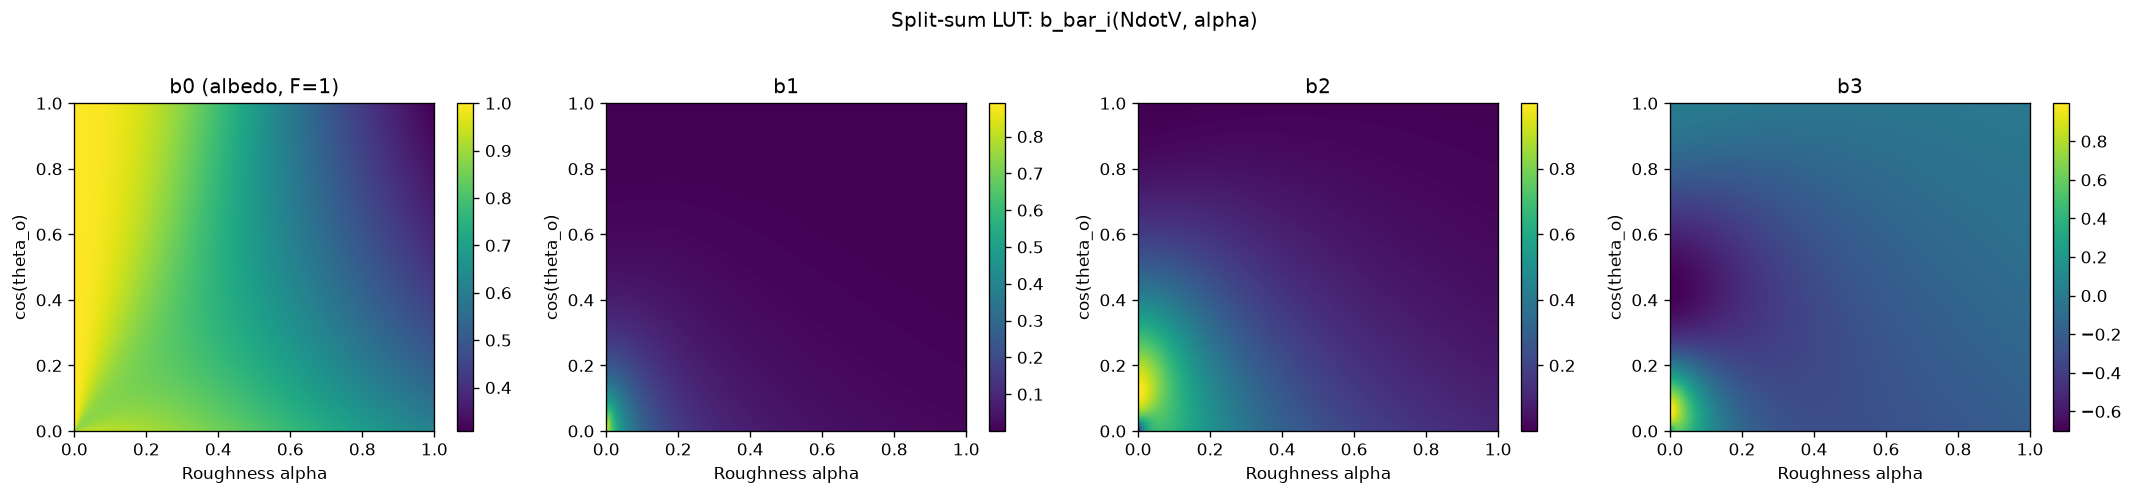
\includegraphics[width=\linewidth]{split_sum.png}
\caption{The preintegrated weights $\bar b_i(\cos\theta_o,\alpha)$.  Channel 0
is the achromatic GGX albedo; channels 1--3 concentrate at grazing view and low
roughness, where the Fresnel curve departs from its normal-incidence value.}
\label{fig:splitsum}
\end{figure}

\subsection{Working in linear sRGB}
\label{sec:prefold}

$\mPhi_i$ acts in XYZ, while a tristimulus renderer (Mitsuba's RGB variants,
Godot) transports linear sRGB.  Rather than converting radiance twice per
pixel, the colour change is folded once into each matrix,
\begin{equation}
  \mPsi_i=\mM_{\text{rgb}\leftarrow\text{xyz}}\;\mPhi_i\;\mM_{\text{xyz}\leftarrow\text{rgb}},
  \label{eq:psi}
\end{equation}
so that $\mM_F$ assembled from $\mPsi_i$ applies directly to sRGB radiance.
\file{audit\_tint.py} verifies the two routes agree to $5.6\times10^{-16}$ for
a single bounce (pure linearity), and \file{export\_godot.py} verifies the
fold inverts back to $\mPhi_i$ to $3.3\times10^{-16}$.

% ======================================================================
\section{Validation renderers}
\label{sec:renderers}

All renders share one scene: a unit gold sphere, GGX with $\alpha=0.05$,
lit by an environment, seen by a narrow 16$^\circ$ camera, 1024$\times$1024
pixels, 2048 samples per pixel, Mitsuba's \code{direct} integrator (one bounce
with next-event estimation and multiple importance sampling).  Three renderers
produce three images per illuminant.

\paragraph{Reference (\file{render\_reference.py}).}  Mitsuba's
\code{llvm\_ad\_spectral} variant with the stock \code{roughconductor} and
gold's $\eta,\kappa$ given as spectral files.  Each ray packet carries four
wavelengths; the film projects onto XYZ with the CMF table of
Section~\ref{sec:norm}.  It serves as ground truth.

\paragraph{Spectral path (\file{render\_ours.py}).}  The same spectral
variant, with a custom Python BSDF that keeps everything of the stock
microfacet model except the Fresnel term, which it replaces per wavelength by
the four-coefficient reconstruction of Section~\ref{sec:coeffs}, solving the
$2\times2$ system on the fly for the wavelengths of each packet.  No reduction
is involved: this isolates the angular decomposition alone.

\paragraph{Reduced-matrix path (\file{render\_ours\_direct.py}).}  The
\code{llvm\_ad\_rgb} variant with a custom integrator that re-implements
\code{direct} (emitter sampling, BSDF sampling, power-heuristic weights) but
replaces the scalar Fresnel multiply by the matrix product
$L_{\text{out}}=\mM_F(\cos\theta_d)\,L_{\text{in}}$ on the actual transported
radiance, using the pre-folded $\mPsi_i$.  It is the real-time formulation.

\paragraph{The $F{=}1$ trick.}  Neither custom path re-implements GGX.  Each
instantiates a stock \code{roughconductor} with a dummy index
($\eta=0,\ \kappa=10^5$, hence $F\approx1$ at all angles) and uses it as an
achromatic geometry term and VNDF sampler, then multiplies by its own Fresnel.
The angle fed to the Fresnel is the half-vector angle
$\cos\theta_d=\wi\!\cdot\!\vh$, recomputed as \code{dot(si.wi, normalize(si.wi + wo))}.
Basis values are gathered from the 1000-entry table at
$\operatorname{round}(999\cos\theta_d)$ in both paths.

\subsection{The reference confound and the four illuminants}
\label{sec:confound}

The Uffizi environment map is an RGB image.  In a spectral variant, Mitsuba
must invent a spectrum for every RGB pixel and does so with Jakob \& Hanika
(2019) upsampling; the reduced path implicitly uses the dual-basis metamer
$\mSd\vc$ instead.  Two arbitrary metamers of the same RGB pixel: the residual
between reference and reduced render mixes the reduction error with a
disagreement that has nothing to do with the material.  The Uffizi comparison
shows this directly: its error map is non-zero on the background, where no
surface is involved (Figure~\ref{fig:cmp-uffizi}).

\file{make\_illuminants.py} therefore produces three deconfounded lighting
conditions, each rendered by all three paths:
\begin{itemize}[nosep]
  \item \textbf{Uffizi, achromatic}: the luminance of the HDRI replicated to
        $R{=}G{=}B$.  Keeps the angular structure; an achromatic pixel maps to
        a near-flat spectrum under both upsamplings.
  \item \textbf{D65}: a constant emitter with the CIE D65 spectral power
        distribution as a file.  Smooth.  Zero upsampling ambiguity.
  \item \textbf{FL1}: the same with CIE FL1, a spiky fluorescent lamp.
\end{itemize}
The two constant-emitter scenes have no environment structure: the sphere is
lit uniformly from every direction, so the renders show a nearly flat disc
against a flat background, as in a furnace test.  This removes geometry from
the comparison and leaves only the material's spectral response, at the cost
of the scene.
The SPD files are normalised so that the spectral film sees luminance $Y=1$
for a perfect reflector, which requires $\int E\,\bar y\,d\lam=\int\bar y\,d\lam$,
not $=1$.

\subsection{Metric}

\file{compare.py} reports per-pixel RMSE on linear HDR values and per-pixel
CIEDE2000 on Reinhard-tonemapped sRGB converted to CIELAB.  The $\dE$ is
display-referred; it is the number quoted everywhere below.  NaN pixels
(present in the spectral reference as isolated black speckles) are zeroed in
all three images before comparison.

% ======================================================================
\section{Results}
\label{sec:results}

\begin{table}[h]\centering\small
\begin{tabular}{@{}llrrrr@{}}
\toprule
 & & \multicolumn{2}{c}{spectral path} & \multicolumn{2}{c}{reduced matrix} \\
Illuminant & Nature & $\dE$ & RMSE & $\dE$ & RMSE \\
\midrule
Uffizi HDRI            & RGB, upsampled (confounded) & 0.020 & 0.0008 & 2.107 & 0.030 \\
Uffizi, achromatic     & RGB, deconfounded           & 0.020 & 0.0008 & 2.036 & 0.029 \\
D65                    & spectral, smooth            & 0.044 & 0.0009 & 2.700 & 0.032 \\
FL1                    & spectral, spiky             & 0.041 & 0.0008 & 0.783 & 0.011 \\
\bottomrule
\end{tabular}
\caption{Mean CIEDE2000 (display-referred) and mean linear-HDR RMSE against
the spectral reference, gold sphere, $\alpha=0.05$, 2048 spp.  Target for the
reduced path was a mean $\dE$ below 1.  All values regenerated from this
repository; they match the original runs to three decimals.}
\label{tab:results}
\end{table}

The spectral path is at the noise floor under every illuminant; its error maps
are black except for the reference's NaN speckles.  The angular decomposition
is therefore not the limiting factor, and the error of the reduced path comes
from the reduction itself.

The reduced path has a systematic, multiplicative tint.  Under D65 the sphere
is a uniform disc and the error map is a uniform $\approx2.7$ over it.  Under
the structured Uffizi lighting the error follows the radiance: highest on the
bright arch reflection, lowest in the dark regions.  Visually the reduced gold
is less saturated and greener than the reference
(Figures~\ref{fig:cmp-uffizi}--\ref{fig:cmp-spectral}).

The dependence on the illuminant runs against intuition: the spiky fluorescent
FL1 is handled three times better than the smooth daylight D65.
Section~\ref{sec:tint} explains why.

\begin{figure}[p]\centering
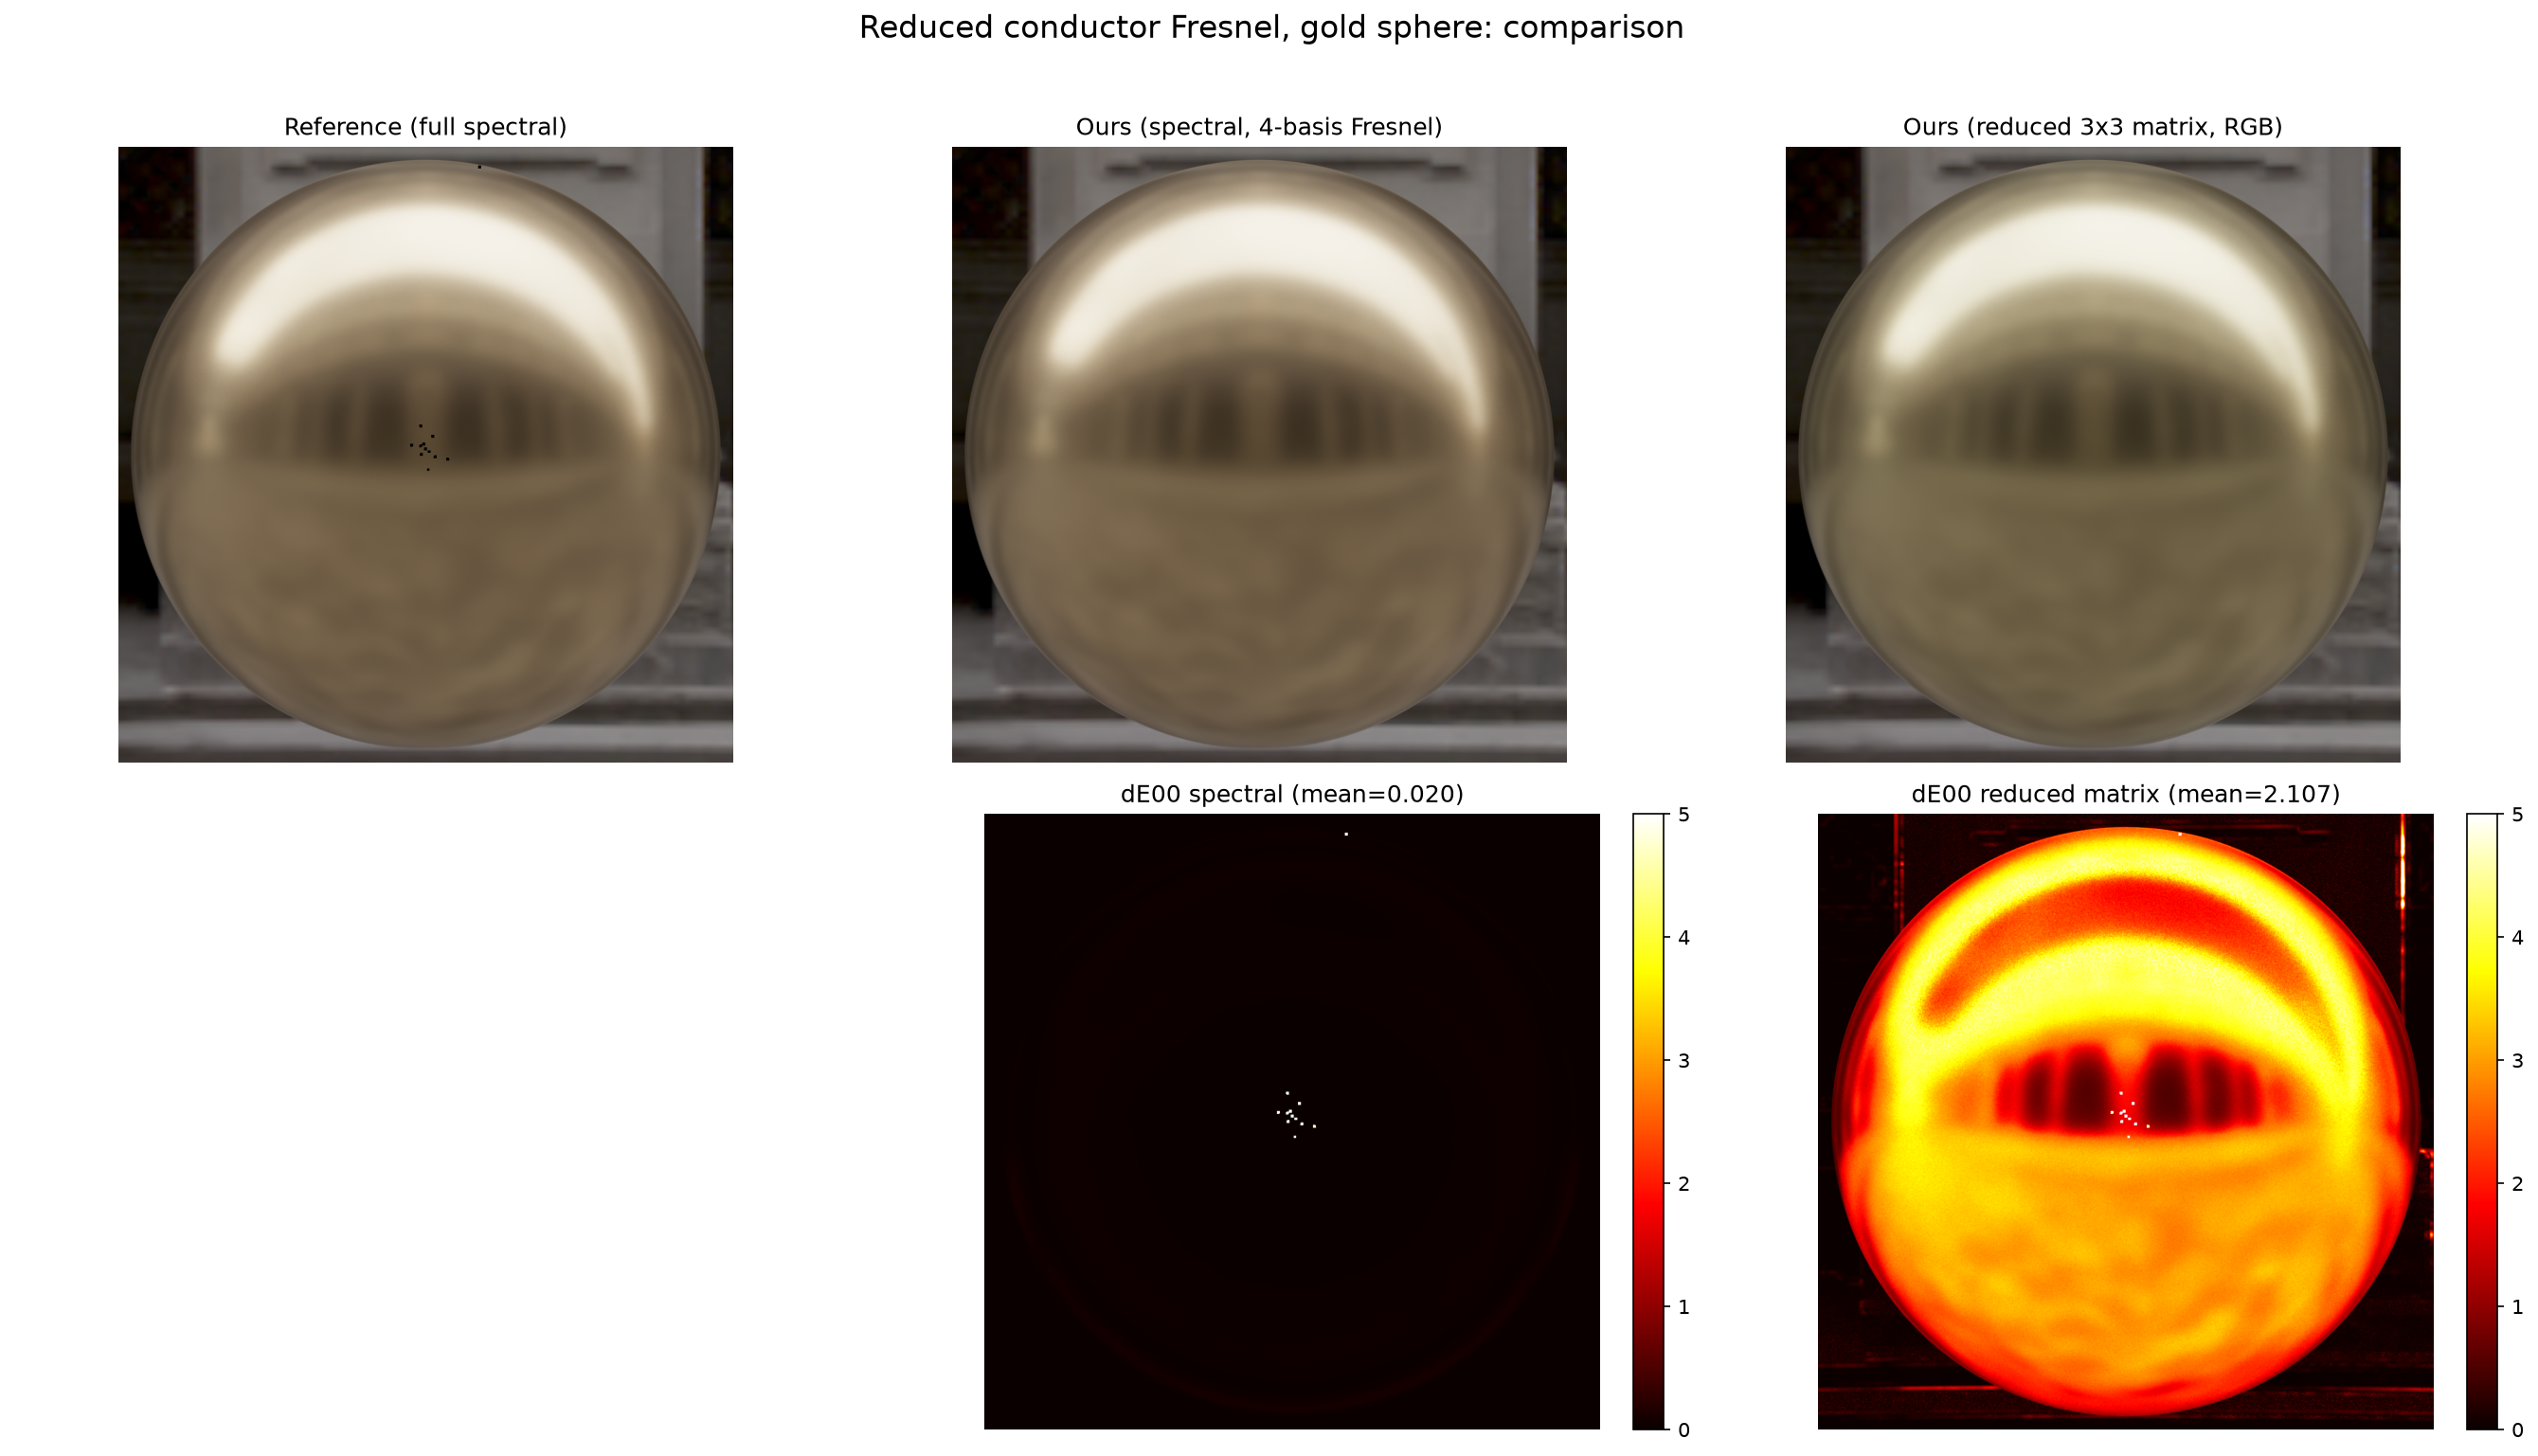
\includegraphics[width=\linewidth]{comparison_uffizi.png}\\[0.6em]
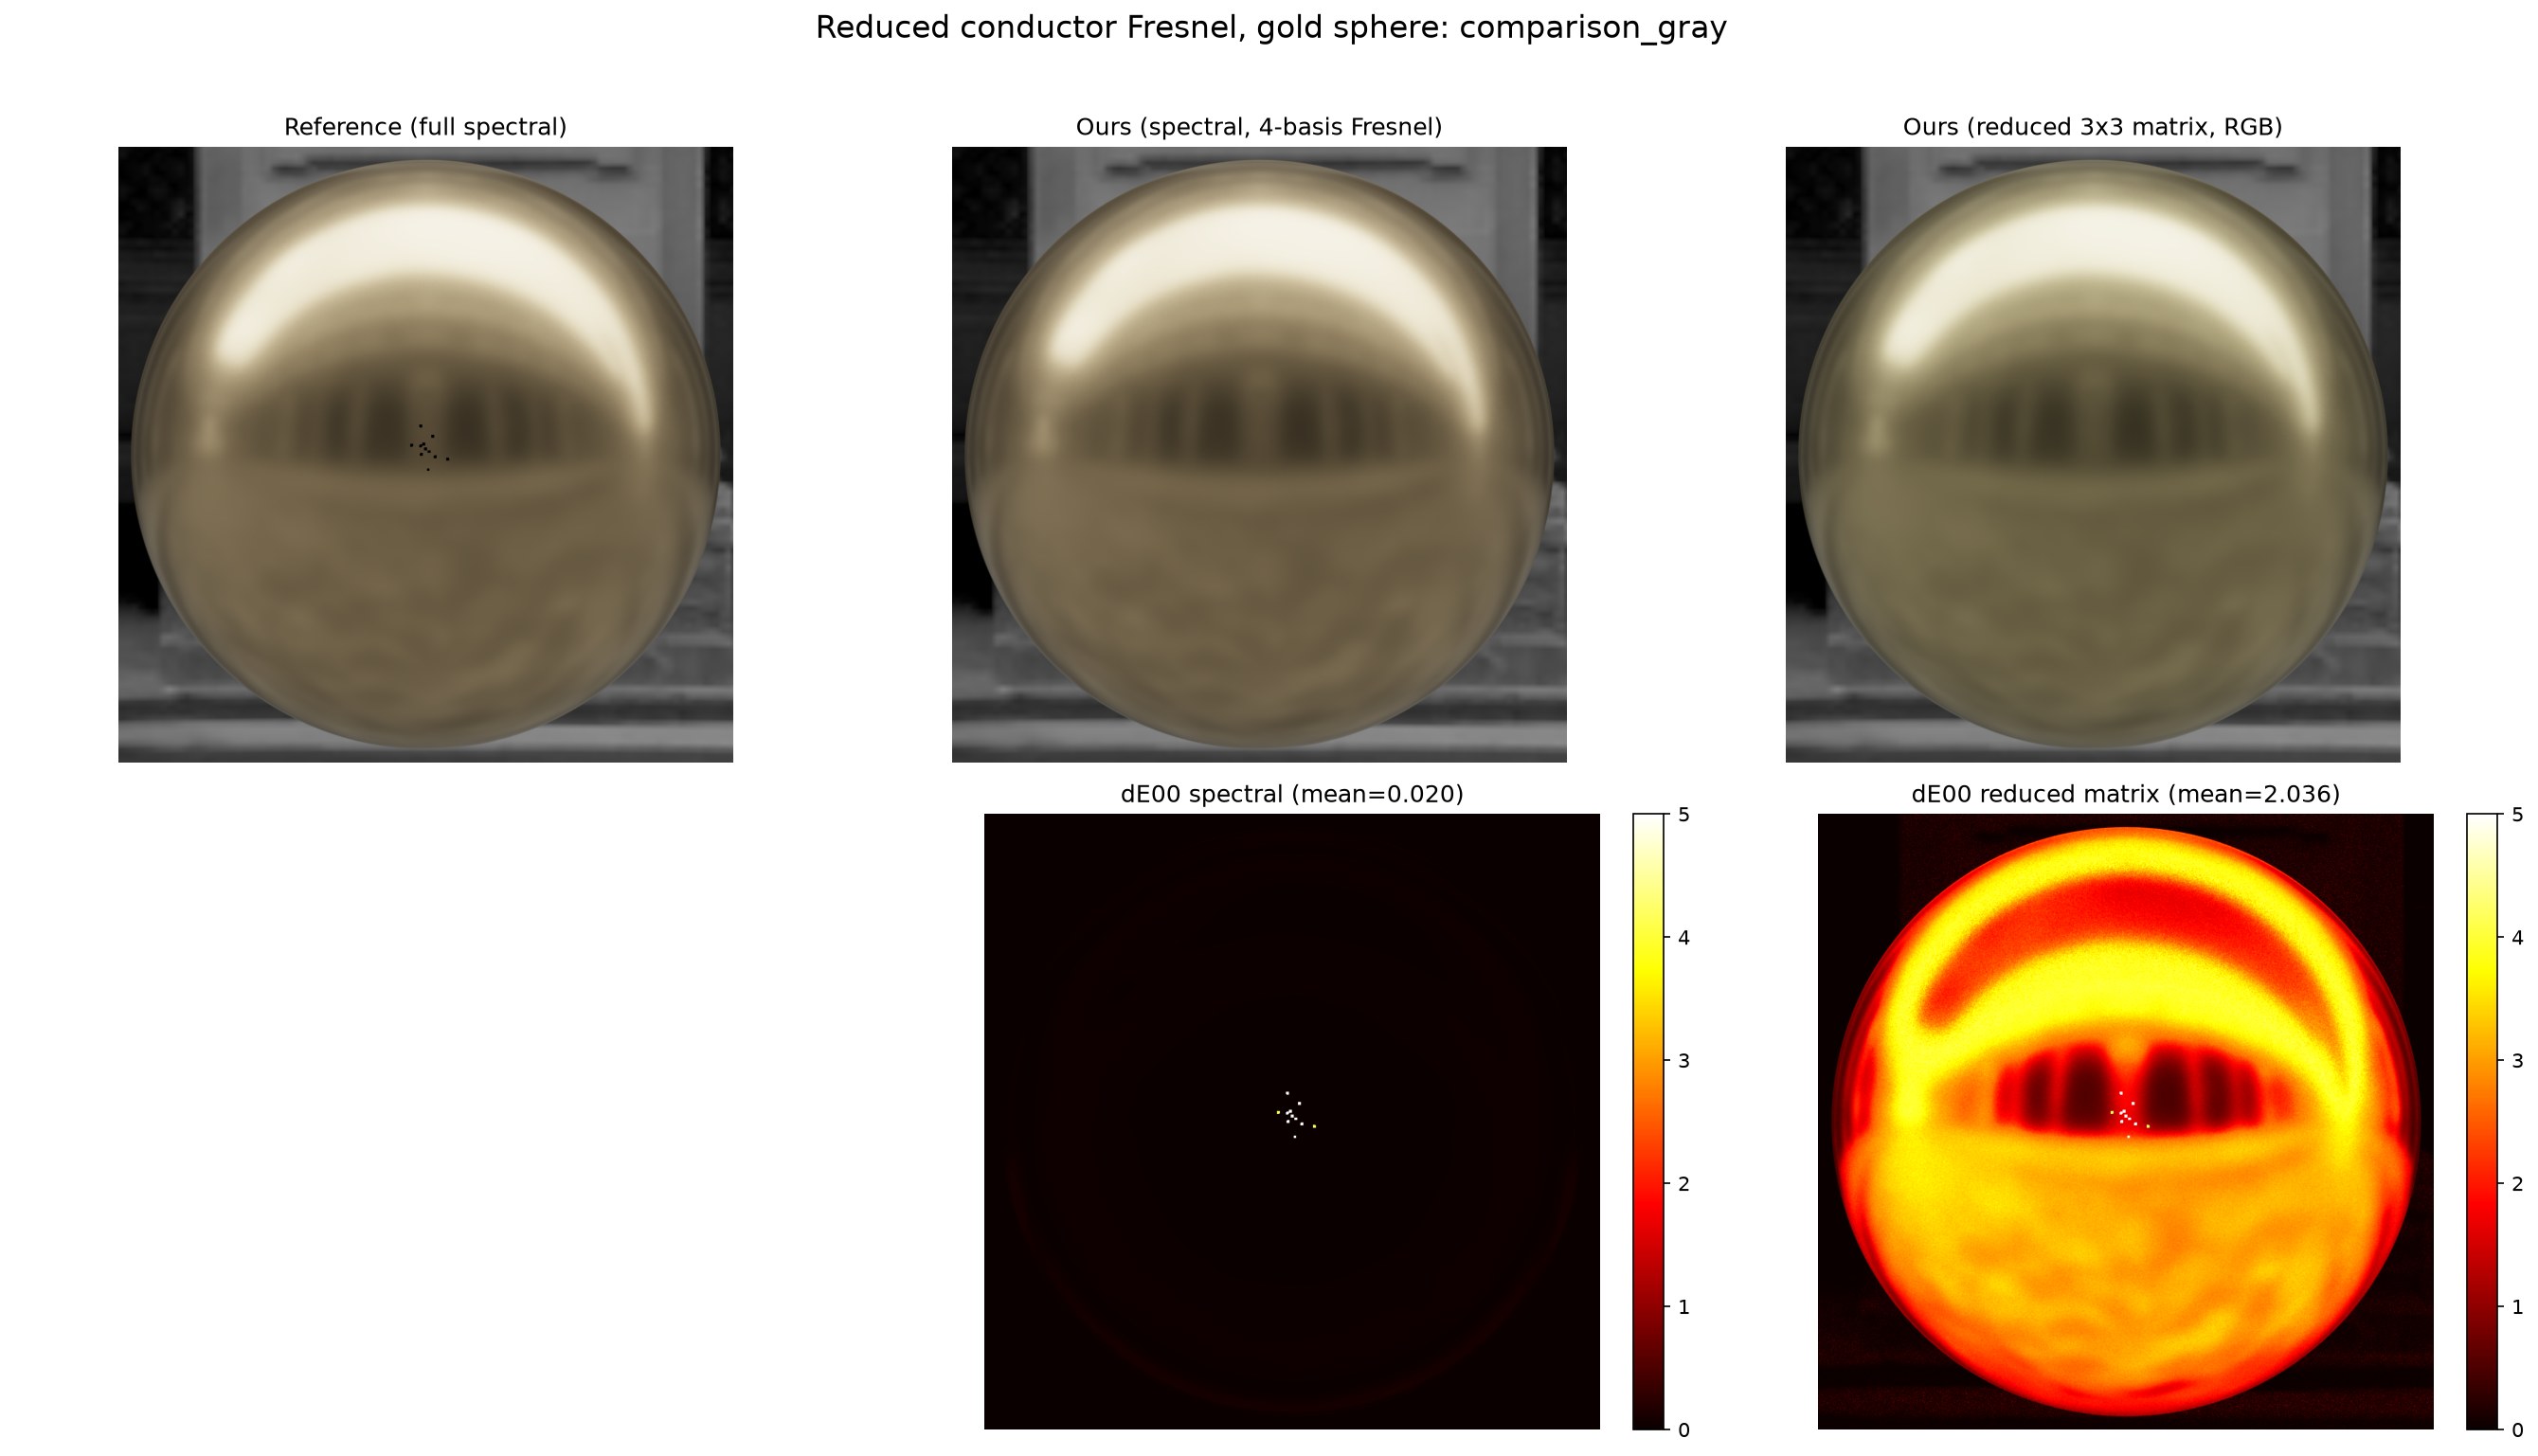
\includegraphics[width=\linewidth]{comparison_gray.png}
\caption{Uffizi HDRI (top) and its achromatic version (bottom).  Left to
right: reference, spectral path, reduced-matrix path; below, $\dE$ maps.  Note
the non-zero background error in the top row, absent in the bottom row.}
\label{fig:cmp-uffizi}
\end{figure}

\begin{figure}[p]\centering
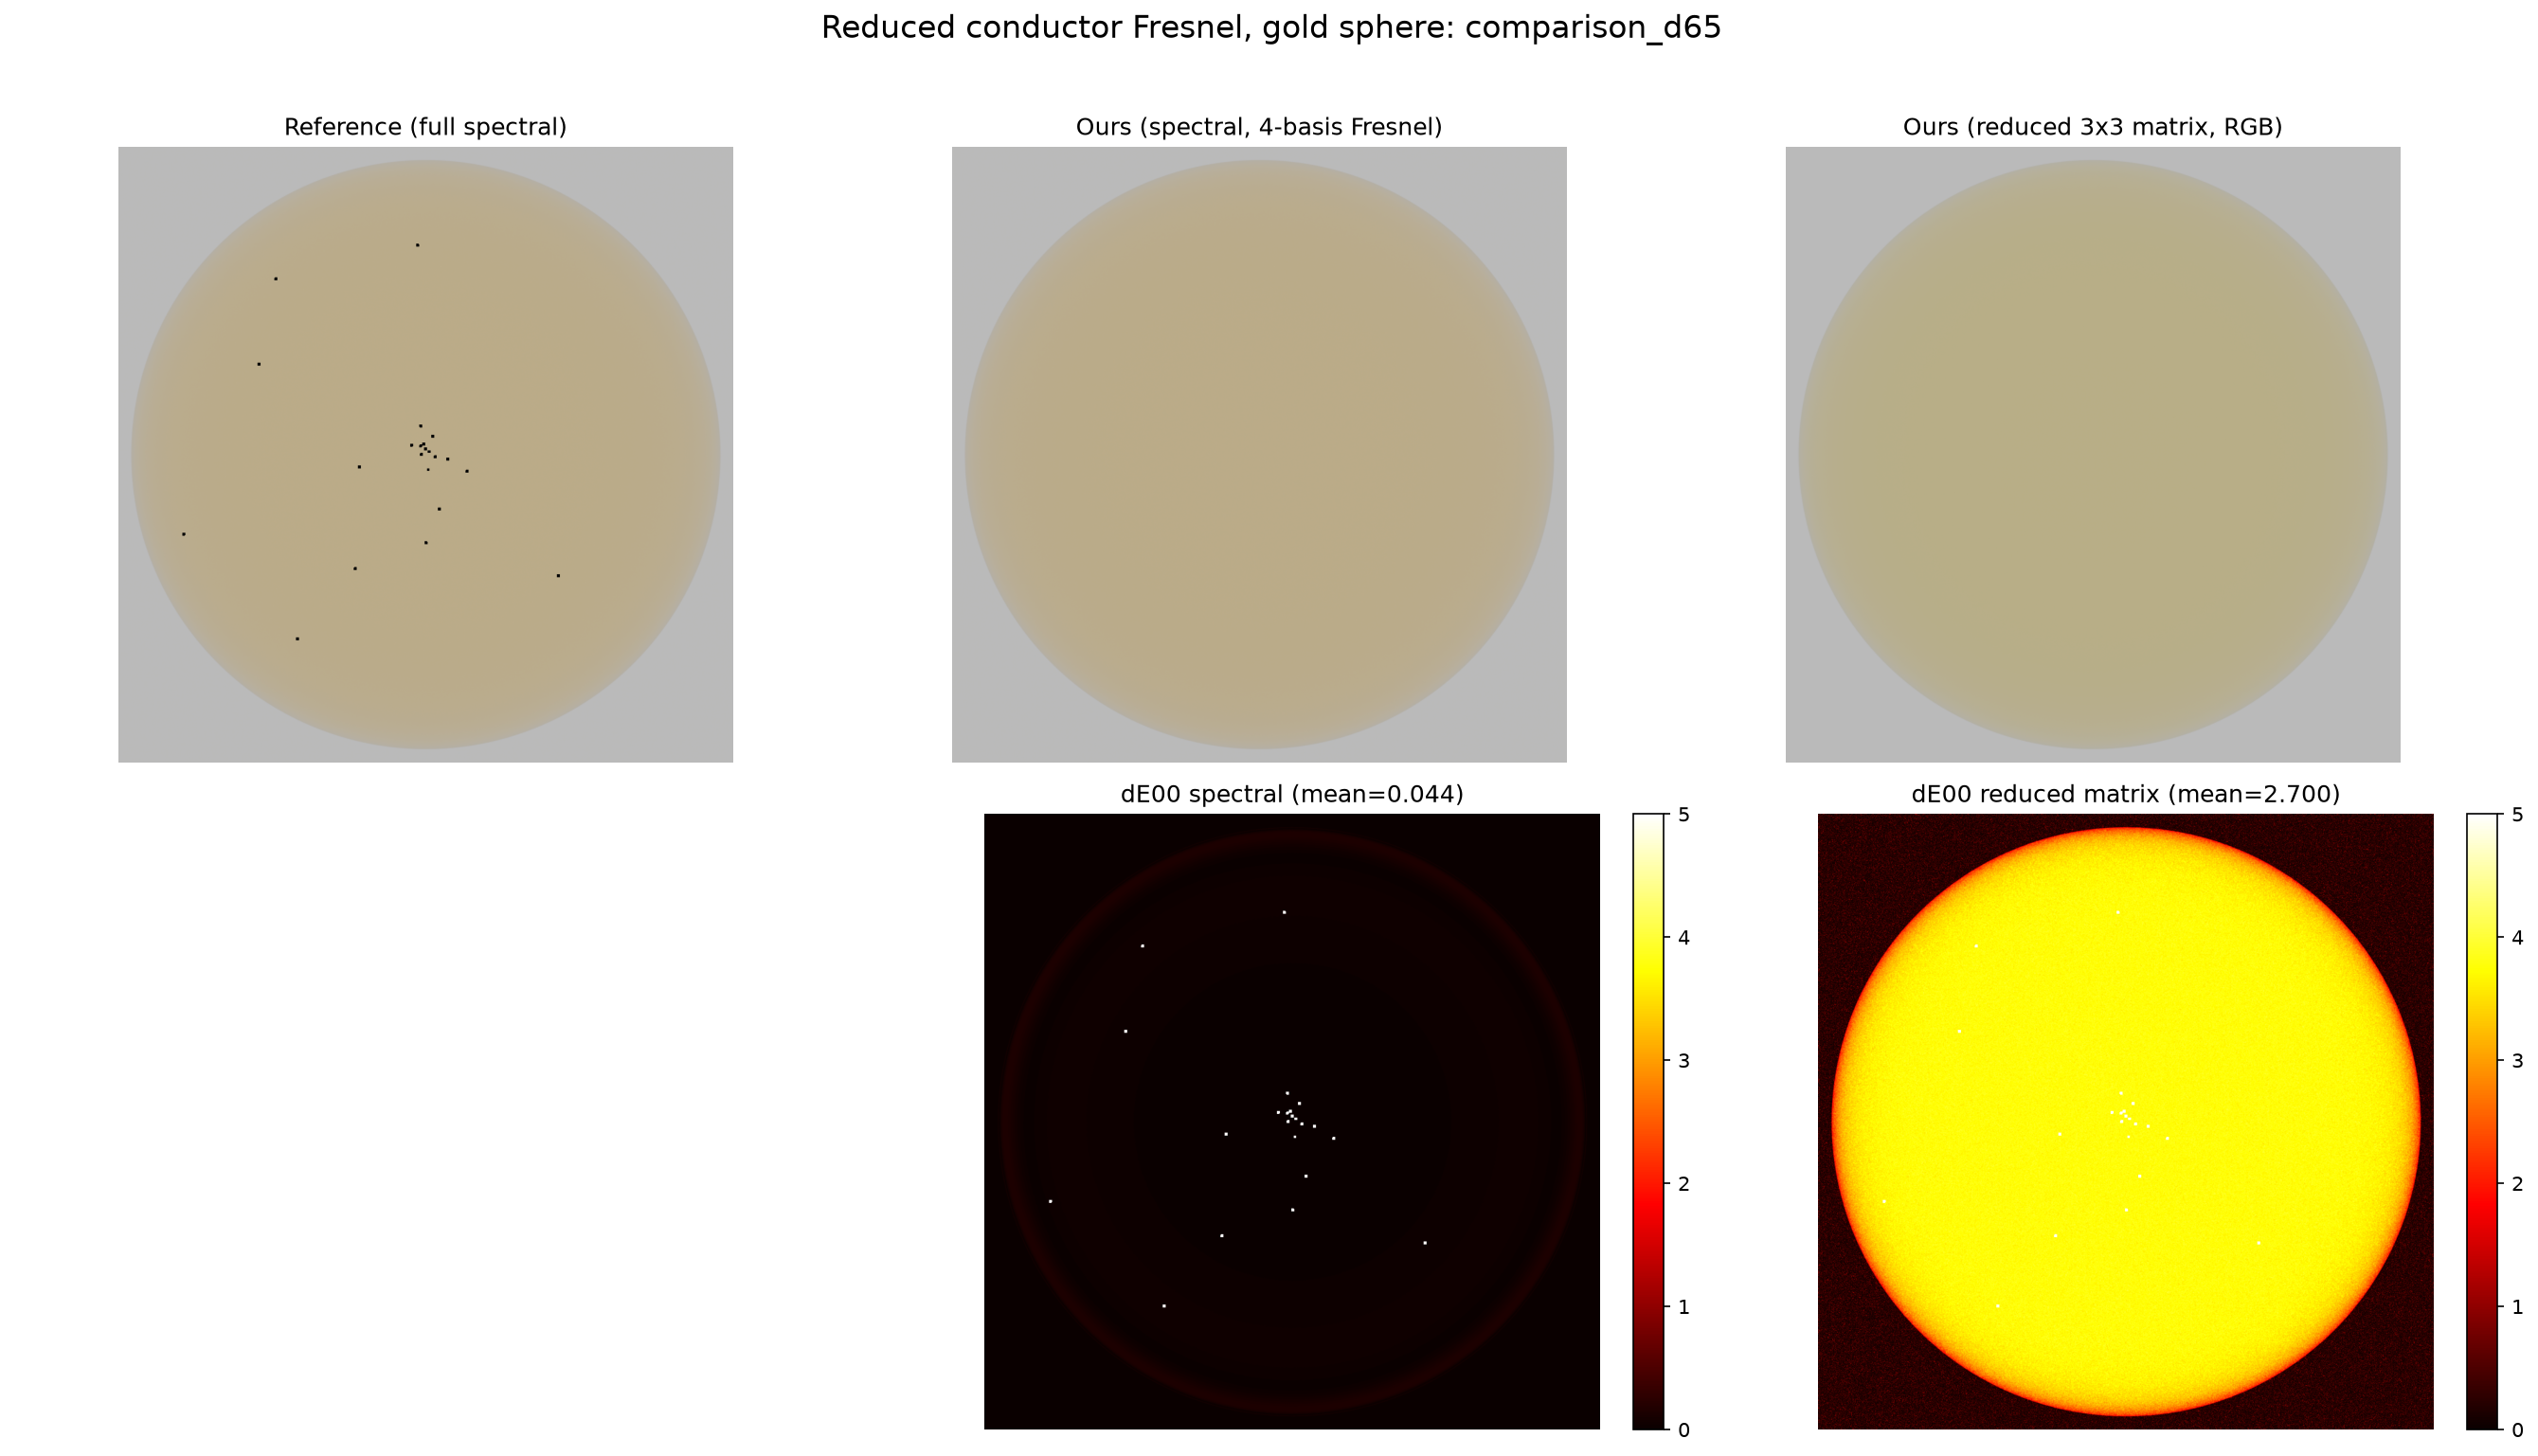
\includegraphics[width=\linewidth]{comparison_d65.png}\\[0.6em]
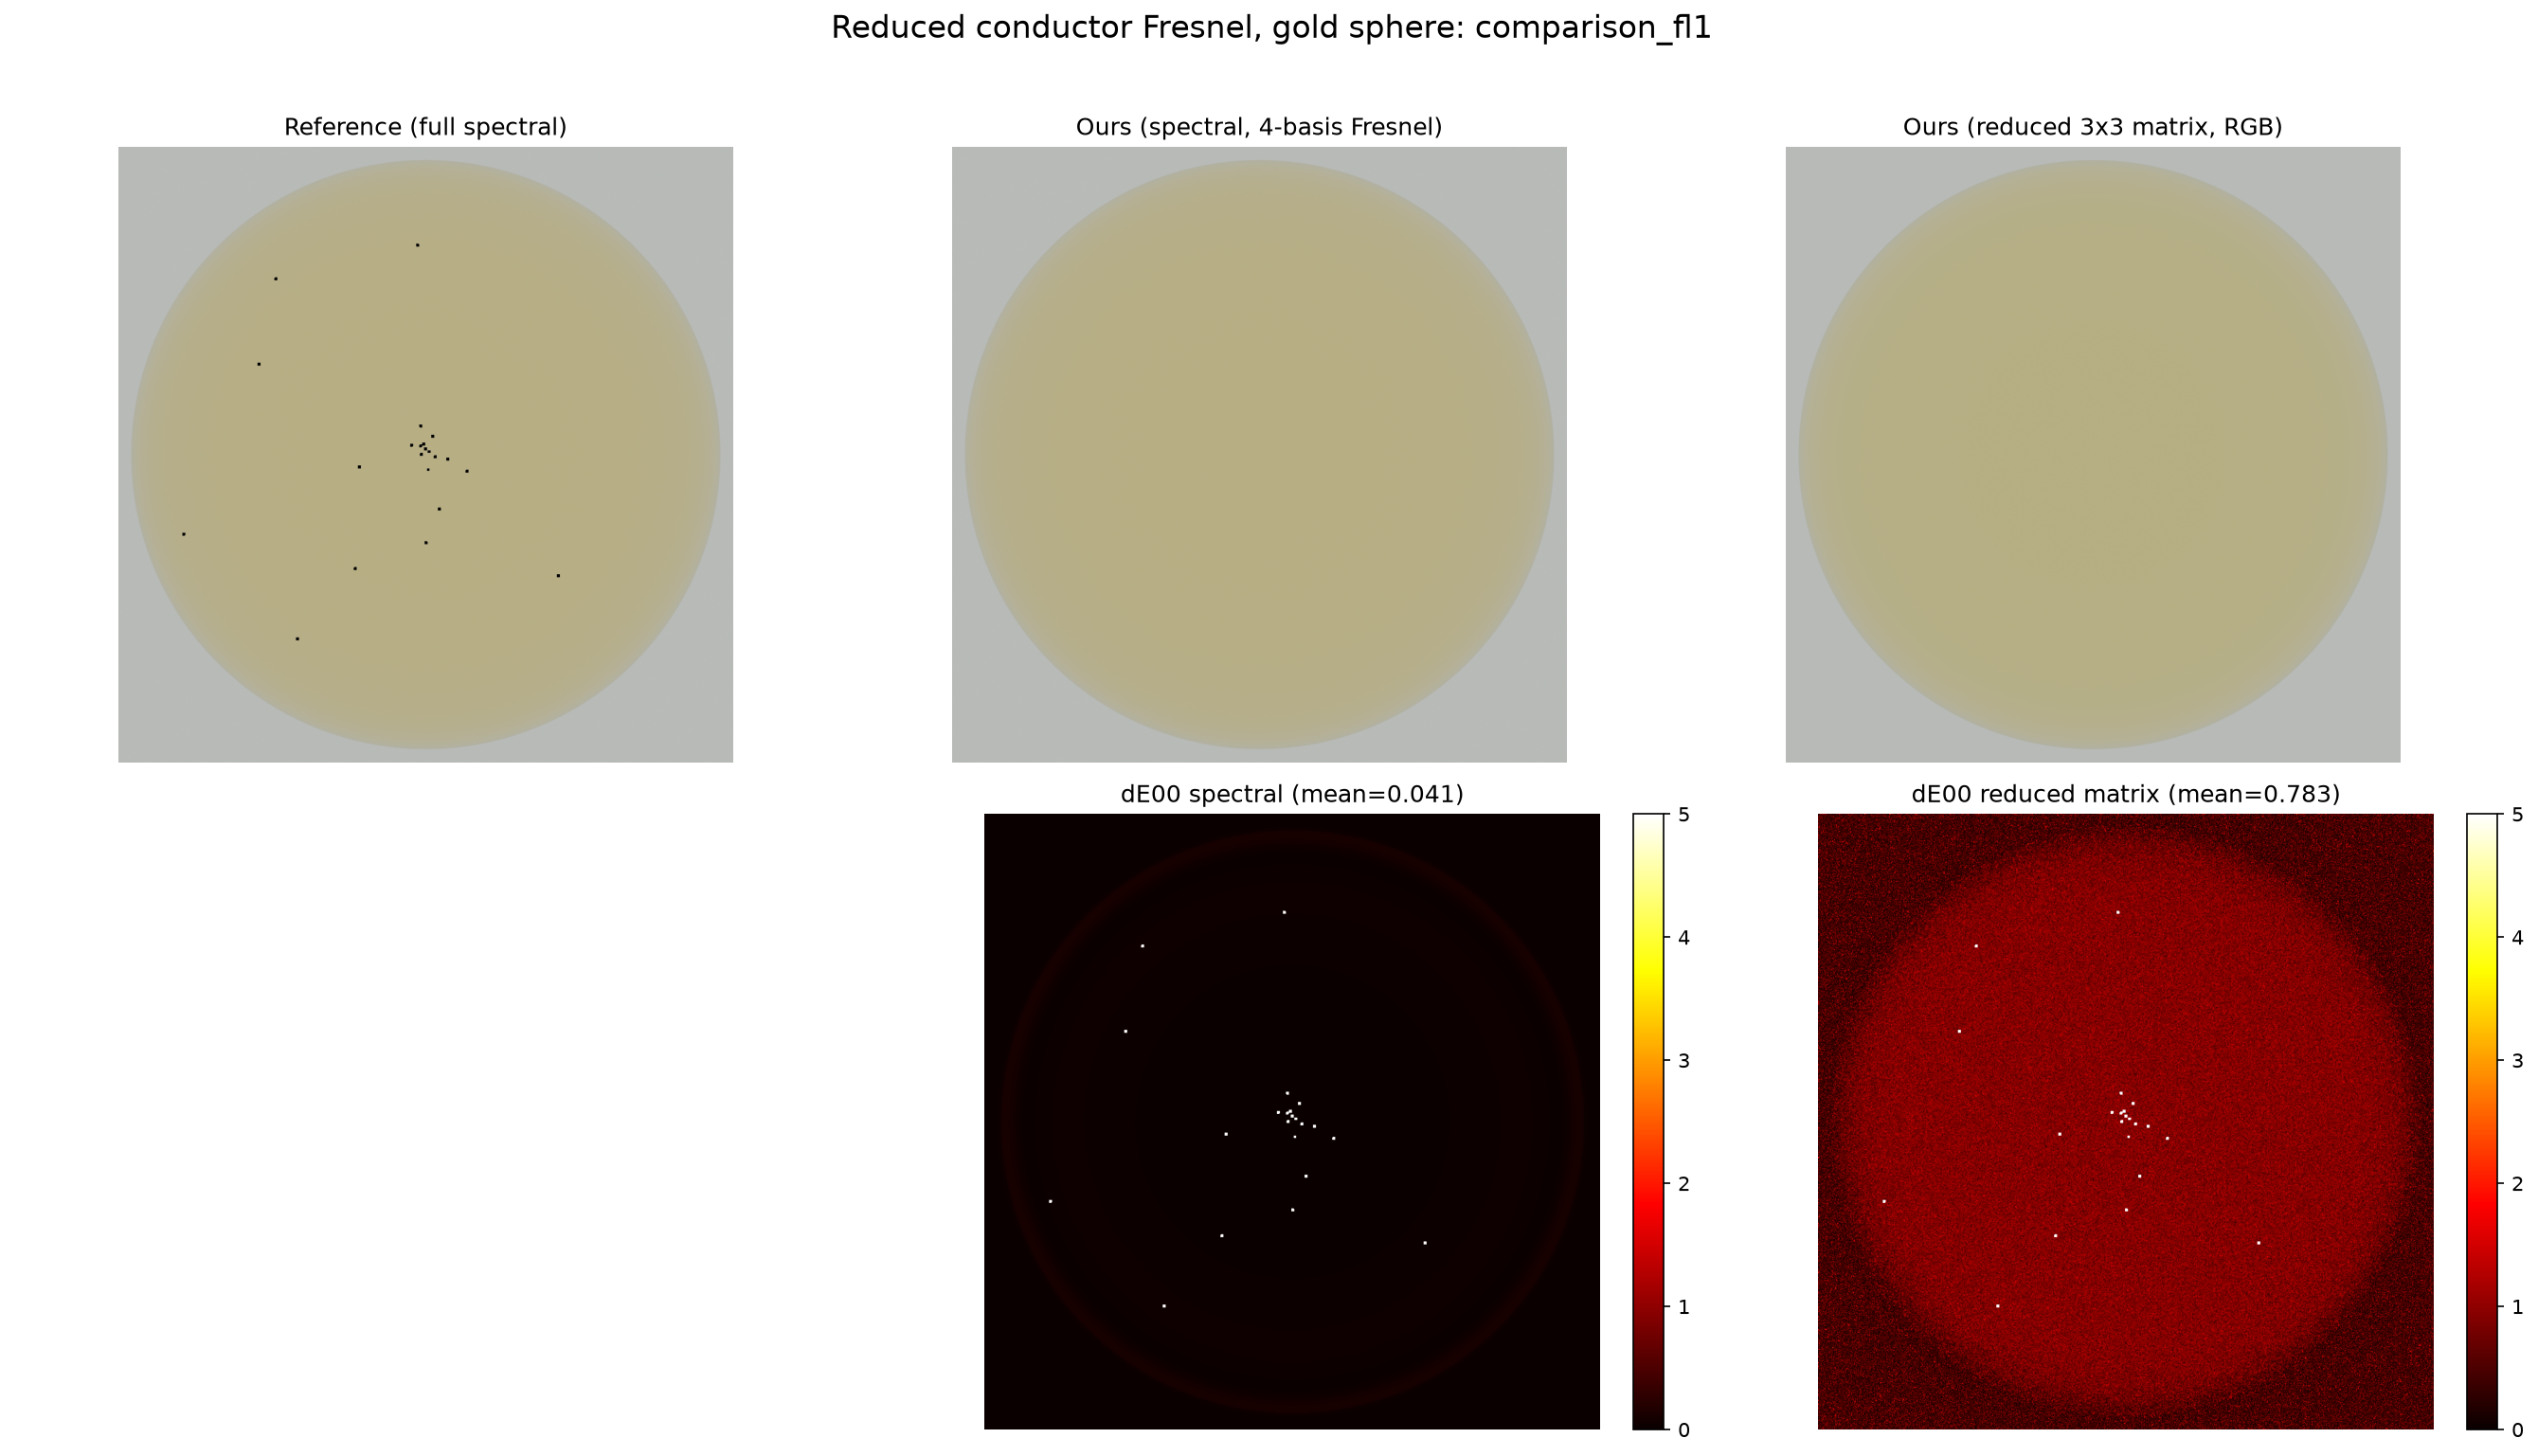
\includegraphics[width=\linewidth]{comparison_fl1.png}
\caption{Natively spectral constant emitters: D65 (top) and FL1 (bottom).
Under D65 the reduced path is uniformly wrong by $\approx2.7$; under FL1 by
$\approx0.8$.}
\label{fig:cmp-spectral}
\end{figure}

% ======================================================================
\section{Diagnosis of the residual tint}
\label{sec:tint}

\file{audit\_tint.py} reproduces the tint offline in pure linear algebra,
without renderer, Monte Carlo or tonemapping, and writes its output to
\file{results/audit\_tint.txt}.  The tint appears there, so it is a property
of the mathematics rather than of the renderer.

\subsection{The tint is the mathematics, not the renderer}

At normal incidence under D65, the exact colour $\mS\transp(F\circ\vE)$ and the
reduced colour $\mPhi\,(\mS\transp\vE)$ convert to linear sRGB as
\[
  \text{exact}=[\,1.025,\ 0.722,\ 0.340\,],\qquad
  \text{reduced}=[\,0.961,\ 0.766,\ 0.329\,],
\]
while the rendered pixels at the sphere centre are
$[1.0226,\,0.7199,\,0.3412]$ and $[0.9563,\,0.7626,\,0.3272]$.  Three-decimal
agreement with a closed-form computation: about $-6\%$ red, $+6\%$ green.

\subsection{Metameric black}

Write the illuminant as the part the basis sees plus the part it cannot:
\begin{equation}
  \vE=\mSd\,\mS\transp\vE+\mB_E,\qquad
  \mB_E=(\mI-\mSd\mS\transp)\,\vE,\qquad \mS\transp\mB_E=0 .
\end{equation}
$\mB_E$ is the \emph{metameric black} of $\vE$ (Wyszecki): invisible to the
observer, and therefore invisible to the reduced pipeline.  The single-bounce
error is exactly
\begin{equation}
  \mS\transp(F\circ\vE)-\mPhi\,\mS\transp\vE
  \;=\;\mS\transp\big(F\circ\mB_E\big),
  \label{eq:black}
\end{equation}
verified numerically to $4\times10^{-16}$.  A flat material leaves $\mB_E$
invisible; gold's wavelength-varying $F$ modulates it back into the visible.
For D65, $\|\mB_E\|/\|\vE\|=0.55$: over half of the illuminant's energy, in
$L_2$, is black to the dual basis.  A spiky spectrum such as FL1 happens to
have less of its energy in that complement, which is why it is handled better.

\subsection{The reconstruction operator is a free design axis}

Nothing in Eq.~\eqref{eq:reduce} forces the reconstruction to be $\mSd$.  Any
$\mR\in\mathbb{R}^{N\times3}$ with $\mS\transp\mR=\mI_3$ gives a valid reduced
operator $\mPhi=\mS\transp\diag(f)\,\mR$, exact on $\operatorname{span}\mR$.
The dual basis is the choice with minimal norm; it is not the choice with
minimal error on the spectra one actually meets.  \file{audit\_tint.py}
compares several, at five angles, against the exact spectral colour
(Table~\ref{tab:audit}).  These $\dE$ values are computed on un-tonemapped
$O(1)$ colours and are \emph{not} numerically comparable to
Table~\ref{tab:results}; only their ranking and the closed-form reproduction
above carry over.

\begin{table}[h]\centering\small
\begin{tabular}{@{}lrrrrrrrr@{}}
\toprule
Reconstruction $\mR$ / baseline & E & A & D50 & D65 & D75 & FL1 & FL2 & FL4 \\
\midrule
{[A]} dual basis $\mSd$ (this work)     & 5.52 & 2.45 & 5.93 & 7.00 & 7.57 & 1.69 & 0.43 & 0.71 \\
{[A4]} same, 4-basis $\mM_F$            & 5.49 & --   & --   & 6.97 & --   & 1.66 & --   & --   \\
{[C]} daylight $S_0S_1S_2$ anchor       & 0.58 & 0.33 & 0.00 & 0.00 & 0.00 & 4.80 & 5.42 & 3.61 \\
{[D]} anchored on D65, FL1, A           & 3.81 & 0.00 & 5.04 & 0.00 & 4.69 & 0.00 & 0.85 & 3.23 \\
{[I]} Mallett--Yuksel sRGB primaries    & 0.00 & 0.37 & 0.54 & 0.99 & 1.27 & 3.83 & 5.14 & 3.64 \\
\addlinespace
{[E]} diagonal, flat-weighted           & 0.00 & 4.44 & 2.47 & 1.24 & 3.67 & 5.29 & 2.36 & 2.83 \\
{[G]} Belcour 2020, RGB-averaged IOR    & 1.51 & 4.72 & 3.86 & 1.55 & 2.61 & 3.87 & 1.33 & 2.63 \\
\bottomrule
\end{tabular}
\caption{Mean $\dE$ over five angles, single bounce, gold, against the exact
spectral colour.  Rows [A]--[I] are matrix operators differing only in
$\mR$; [E] and [G] are per-channel (diagonal) baselines of the kind engines
use.  Exact zeros are exact by construction.}
\label{tab:audit}
\end{table}

The [A] and [A4] rows agree to $0.03$, so the angular decomposition adds
nothing to the error, in line with Section~\ref{sec:results}.  An $\mR$
anchored on the CIE daylight components makes the reduction exact on every
daylight illuminant and near-exact on the flat one, at the same runtime cost,
since only the $\mPhi_i$ change.  It is worse on fluorescent lamps, where the
dual basis does better.  No single $3$-dimensional $\mR$ is good everywhere;
the choice fixes the family of illuminants on which the reduction is exact.

\subsection{Why a matrix, and not a diagonal}

The [E] and [G] rows already show that a per-channel Fresnel is wrong by
$1$--$5$ $\dE$ once the illuminant is not the one it was averaged under.  The
decisive comparison is over depth.  Ward's prefiltering (row [F] of the audit)
sets $\rho_k=(\mS\transp(F\circ\vE))_k/(\mS\transp\vE)_k$ and is therefore
\emph{exact at one bounce, by construction}.  Table~\ref{tab:bounce} iterates
each operator three times at $\cos\theta=0.707$.

\begin{table}[h]\centering\small
\begin{tabular}{@{}llrrrr@{}}
\toprule
Operator & Illuminant & 1 bounce & 2 bounces & 3 bounces & $\operatorname{cond}\mR$ \\
\midrule
{[A]} dual basis           & D65 & 8.28 & 9.25 & 8.10  & 1.0 \\
{[C]} daylight anchor      & D65 & 0.00 & 1.14 & 1.92  & 8.4 \\
{[I]} Mallett--Yuksel      & D65 & 1.12 & 0.32 & 1.47  & --  \\
{[F]} diagonal, Ward-prefiltered & D65 & 0.00 & 4.77 & 9.83 & -- \\
{[E]} diagonal, flat       & D65 & 1.37 & 2.70 & 6.81  & -- \\
{[D]} anchored on three lamps & D65 & 0.00 & 7.32 & 14.72 & 49.7 \\
{[H]} PCA of ten lamps     & D65 & 0.59 & 15.91 & 49.29 & 113 \\
\addlinespace
{[A]} dual basis           & FL1 & 2.12 & 2.15 & 1.47  & 1.0 \\
{[C]} daylight anchor      & FL1 & 5.83 & 8.52 & 8.93  & 8.4 \\
{[F]} diagonal, Ward-prefiltered & FL1 & 0.00 & 5.91 & 11.92 & -- \\
\bottomrule
\end{tabular}
\caption{$\dE$ after $n$ applications of the operator, against $n$ exact
spectral reflections.  The diagonal prefilter is exact once and degrades
linearly; the smooth-anchored matrix stays below 2; naively anchored
reconstructions are ill-conditioned and diverge.}
\label{tab:bounce}
\end{table}

The matrix formulation is what allows an anchored reconstruction to survive
transport depth: the off-diagonal terms carry the inter-channel coupling that a
diagonal operator fabricates at the second bounce.  It is also a warning: an
anchor chosen by fitting a handful of lamps ([D], [H]) has a badly conditioned
$\mR$ and explodes, so the smoothness of the anchor family matters more than
its fit at one bounce.

% ======================================================================
\section{Export to the engine}
\label{sec:godot}

\file{export\_godot.py} writes \file{results/godot\_gold.json} with the four
pre-folded $\mPsi_i$ (row-major, applied as $\text{out}_r=\sum_c\Psi_{rc}L_c$)
and the four basis arrays $b_i$ on the uniform 1000-point $\cos\theta$ grid.
The export also fixes the following:
\begin{itemize}[nosep]
  \item The basis is shipped as the \emph{full sampled arrays}, packed into a
        $1000\times1$ RGBA32F texture and fetched at $u=\cos\theta$, rather than
        as a polynomial fit.  $b_3\in[-0.70,\,1.0]$ is negative over most of its
        range, so an 8-bit texture would silently clamp it.
  \item A Godot \code{Basis} bound to a \code{mat3} uniform reads columns;
        the row-major JSON must be uploaded column by column.
\end{itemize}
Before writing, the script checks that the fold of Eq.~\eqref{eq:psi} inverts
back to $\mPhi_i$ ($3.3\times10^{-16}$) and that the four-basis assembly
$\sum_i b_i\mPhi_i$ agrees with the exact reduced operator
$\mS\transp\diag(F(\cos\theta))\,\mSd$ recomputed from the IOR at five angles
(maximum entry difference $2.2\times10^{-3}$, the four-basis fit error).  It
exits non-zero if either fails.  The runtime cost is one RGBA fetch, four
$3\times3$ multiply-adds and one matrix-vector product per pixel.

% ======================================================================
\section{Limitations and caveats}
\label{sec:limits}

\begin{enumerate}
  \item \textbf{The reduced path misses its target.}  Mean $\dE$ of
        $2.0$--$2.7$ under smooth illuminants against a target below 1.  The
        cause is understood (Section~\ref{sec:tint}) and a fix is identified
        (a smooth-anchored $\mR$) but \emph{not implemented in the render
        pipeline}: all rendered results use the dual basis.  Regenerating
        $\mPhi_i$ with the daylight anchor and re-rendering is the immediate
        next step.
  \item \textbf{The split-sum LUT is unvalidated in a render.}  It inherits
        every limit of the split-sum approximation: bilinear blur at low
        $\alpha$ and grazing view, per-texel Monte Carlo variance, isotropic
        roughness only, the separable $G_2\approx G_1G_1$ error frozen into
        the table, single scattering (GGX energy loss at high roughness), and
        the distant-lighting assumption that integrates $\wi$ out.
  \item \textbf{The reference has NaN pixels.}  Isolated black speckles in the
        spectral reference (absent in the spectral path, which shares its
        geometry code) are zeroed before comparison and inflate the maximum
        $\dE$, not the mean.  Their origin in Mitsuba's spectral
        \code{roughconductor} at low roughness was not investigated.
  \item \textbf{Two $\dE$ conventions.}  \file{compare.py} measures
        tonemapped, display-referred colour over the whole image including
        the background; \file{audit\_tint.py} measures un-tonemapped colour
        at five angles on the material alone.  Magnitudes do not transfer
        between Tables~\ref{tab:results} and~\ref{tab:audit}.
  \item \textbf{The Uffizi comparison is confounded} by the upsampling
        disagreement of Section~\ref{sec:confound}; its background error is
        the proof.  Quote the three deconfounded rows.
  \item \textbf{Single bounce in the renderer.}  \file{render\_ours\_direct.py}
        applies the matrix once and clamps negatives in sRGB per bounce; a
        path-traced extension should carry the throughput as an ordered
        product of matrices in XYZ and clamp only at the sensor.
        Table~\ref{tab:bounce} is offline algebra, not a render.
  \item \textbf{The basis is not re-derived.}  It is the authors' published
        table, read verbatim; its training corpus (99\% dielectrics, 1\%
        conductors) bounds its fidelity on exotic metals.
  \item \textbf{Normalisation differs from the fluorescence repository}
        (Section~\ref{sec:norm}).  Do not reuse one repository's $\mS$ or
        $\mSd$ in the other.
  \item \textbf{Prior art.}  Reduced-coordinate transport with matrix-valued
        throughput is already in Fichet et al.\ (2024, \S4.1) and, earlier, in
        Peercy (1993).  What is new here is only the angular factorisation
        $\mM_F(\theta)=\sum_ib_i(\theta)\mPhi_i$ and its matrix-valued
        split-sum.
\end{enumerate}

% ======================================================================
\section{Reproduction}
\label{sec:repro}

\begin{verbatim}
make venv            # python3 -m venv .venv ; pip install -r requirements.txt
make precompute      # load_ior, extract_basis, compute_coeffs, compute_cmf, compute_phi
make check           # check_conventions + export_godot (both exit 1 on failure)
make audit           # audit_tint -> results/audit_tint.txt
make illuminants     # scene/uffizi_gray.exr, scene/illum_{d65,fl1}.spd
make render          # 12 renders: {reference, ours, ours_direct} x {uffizi, gray, d65, fl1}
make compare         # 4 comparison figures with their Delta-E numbers
make splitsum        # results/split_sum.npy and its figure (Monte Carlo, all cores)
make doc             # this document (latexmk), after `make figures`
\end{verbatim}
All scripts resolve \file{data/}, \file{scene/} and \file{results/} relative
to their own location (\file{scripts/\_paths.py}) and run from any directory.
Renders are deterministic for a fixed Mitsuba version and seed.  Pinned
versions: Python 3.12, Mitsuba 3.9.0, Dr.Jit 1.4.0, numpy 2.5.0, scipy
1.18.0, matplotlib 3.11.0, colour-science 0.4.7, imageio 2.37.3, scikit-image
0.26.0, pandas 3.0.3, joblib 1.5.3.  The \file{.exr} renders and the
achromatic environment map are not committed; every PNG and every small
artefact in \file{results/} is.

% ======================================================================
\appendix
\section{File map}

\begin{table}[h]\centering\small
\begin{tabular}{@{}lp{8.6cm}@{}}
\toprule
Path & Role \\
\midrule
\file{scripts/load\_ior.py}            & Section~\ref{sec:fresnel}; gold $\eta,\kappa$ on the 1\,nm grid \\
\file{scripts/extract\_basis.py}       & Section~\ref{sec:basis}; $b_0..b_3$ and the probe angles from the authors' table \\
\file{scripts/compute\_coeffs.py}      & Section~\ref{sec:coeffs}; $c_i(\lam)$, fit check \\
\file{scripts/compute\_cmf.py}         & Section~\ref{sec:norm}; $\mS$, $\mSd$ \\
\file{scripts/compute\_phi.py}         & Eq.~\eqref{eq:phi}; $\mPhi_0..\mPhi_3$ \\
\file{scripts/compute\_split\_sum.py}  & Section~\ref{sec:splitsum}; $\bar b_i$ LUT \\
\file{scripts/check\_conventions.py}   & Section~\ref{sec:norm}; CMF and matrix agreement with Mitsuba \\
\file{scripts/export\_godot.py}        & Section~\ref{sec:godot}; $\mPsi_i$, basis, checks \\
\file{scripts/audit\_tint.py}          & Section~\ref{sec:tint}; every number in Tables~\ref{tab:audit}--\ref{tab:bounce} \\
\file{scripts/make\_illuminants.py}    & Section~\ref{sec:confound}; deconfounded lighting assets \\
\file{scripts/render\_reference.py}    & Section~\ref{sec:renderers}; spectral ground truth \\
\file{scripts/render\_ours.py}         & Section~\ref{sec:renderers}; spectral path, four-basis Fresnel \\
\file{scripts/render\_ours\_direct.py} & Section~\ref{sec:renderers}; reduced-matrix path \\
\file{scripts/compare.py}              & Section~\ref{sec:results}; metrics and figures \\
\file{scripts/fresnel\_tools.py}       & exact conductor Fresnel (authors' helper, reduced) \\
\file{data/gold\_refractive\_index.csv} & complex IOR of gold \\
\file{data/belcour2020/fresnel\_curves.hpp} & the universal basis table (authors' Mitsuba plugin) \\
\file{scene/}                          & Mitsuba scenes, spectral IOR and illuminant files, Uffizi HDRI \\
\bottomrule
\end{tabular}
\end{table}

\section{Symbols}

\begin{table}[h]\centering\small
\begin{tabular}{@{}lll@{}}
\toprule
Symbol & Shape & Meaning \\
\midrule
$\mS$, $\mSd$          & $N\times3$    & CMF basis (common $\bar y$ normalisation) and its dual \\
$\mR$                  & $N\times3$    & any reconstruction with $\mS\transp\mR=\mI$ \\
$\eta(\lam),\kappa(\lam)$ & $N$        & real and imaginary index of gold \\
$F(\theta,\lam)$       & scalar        & exact conductor Fresnel \\
$b_i(\cos\theta)$      & 1000 samples  & universal angular bases, $i=0..3$ \\
$c_i(\lam)$            & $N$           & per-wavelength coefficient of $b_i$ \\
$\mPhi_i$, $\mPsi_i$   & $3\times3$    & reduced coefficient operator in XYZ, and pre-folded in linear sRGB \\
$\mM_F(\theta)$        & $3\times3$    & assembled reduced Fresnel, Eq.~\eqref{eq:MF} \\
$\bar b_i(\cos\theta_o,\alpha)$ & $256\times256$ & preintegrated weights, Eq.~\eqref{eq:bbar} \\
$\mB_E$                & $N$           & metameric black of illuminant $\vE$ \\
\bottomrule
\end{tabular}
\end{table}

\section*{References}
\begin{itemize}[nosep]
  \item A.~Fichet, L.~Belcour, P.~Barla. \emph{Non-Orthogonal Reduction for
        Rendering Fluorescent Materials in Non-Spectral Engines.} Computer
        Graphics Forum, 2024.
  \item L.~Belcour, M.~Bati, P.~Barla. \emph{Bringing an Accurate Fresnel to
        Real-Time Rendering: a Preintegrable Decomposition.} SIGGRAPH Talks,
        2020.
  \item W.~Jakob, J.~Hanika. \emph{A Low-Dimensional Function Space for
        Efficient Spectral Upsampling.} Computer Graphics Forum, 2019.
  \item B.~Karis. \emph{Real Shading in Unreal Engine 4.} SIGGRAPH Courses,
        2013.
  \item E.~Heitz. \emph{Sampling the GGX Distribution of Visible Normals.}
        JCGT, 2018.
  \item G.~Ward, E.~Eydelberg-Vileshin. \emph{Picture Perfect RGB Rendering
        Using Spectral Prefiltering and Sharp Color Primaries.} EGWR, 2002.
  \item I.~Mallett, C.~Yuksel. \emph{Spectral Primary Decomposition for
        Rendering with sRGB Reflectance.} EGSR, 2019.
  \item M.~S.~Peercy. \emph{Linear Color Representations for Full Spectral
        Rendering.} SIGGRAPH, 1993.
  \item G.~Wyszecki, W.~S.~Stiles. \emph{Color Science: Concepts and Methods,
        Quantitative Data and Formulae.} Wiley, 2nd ed.
\end{itemize}

\end{document}
